\documentclass[12pt,a4paper]{article}% 

\usepackage[a4paper,margin=1in]{geometry}
\usepackage{kbordermatrix}
\usepackage{amsmath}
\usepackage{pgfplots}
\usepackage{mathtools}
\usepackage{blindtext}
\usepackage{graphicx}
\usepackage{enumitem}
\usepackage{xcolor}
\usepackage{tikz}
\usepackage{siunitx}
\usepackage{algorithm}
\usepackage{textcomp}
\usepackage[noend]{algorithmic}
\usepackage{listings}
	\lstset{
		frame=tb, % draw a frame at the top and bottom of the code block
		tabsize=4, % tab space width
		showstringspaces=false, % don't mark spaces in strings
		numbers=left, % display line numbers on the left
		commentstyle=\color{green}, % comment color
		keywordstyle=\color{blue}, % keyword color
		stringstyle=\color{red} % string color
	}

\usepackage [english]{babel}
\usepackage [autostyle, english = american]{csquotes}
\MakeOuterQuote{"}
\usepackage{pgfplots,amsmath}
\pgfplotsset{compat=1.12}



\newcommand{\TITLE}[1]{\item[#1]}
\renewcommand{\algorithmiccomment}[1]{$/\!/$ \parbox[t]{4.5cm}{\raggedright #1}}
\newbox\fixbox
\renewcommand{\algorithmicdo}{\setbox\fixbox\hbox{\ {} }\hskip-\wd\fixbox}
\newcommand{\algcost}[2]{\strut\hfill\makebox[1.5cm][l]{#1}\makebox[4cm][l]{#2}}
\usetikzlibrary{arrows,automata,positioning}
\usetikzlibrary{arrows.meta}
\usetikzlibrary{calc}

\pgfmathsetseed{3}
\newcommand*{\Comb}[2]{{}^{#1}C_{#2}}

\begin{document}
	
	
	\begin{titlepage}
	\title{
\includegraphics[width=0.38 \textwidth]{./images/NIT_Silchar_logo.png}\\\textbf{\large NATIONAL INSTITUTE OF TECHNOLOGY, SILCHAR}\\\textbf{{\large Department of Computer Science and Engineering}}\\\bigskip {\large Project Report on,}\\\bigskip\textbf{{\normalsize "DATA TRANSMISSION ANALYSIS AND SIMULATION APPLYING AMPLITUDE/FREQUENCY MODULATION AND EFFECTS OF ATTENUATION ON THE TRANSMITTED SIGNAL." }}}
	%\author{Subject : SDC \\\\ Submitted by,\\Name : \\Scholar ID : }
	\date{\today}
	\clearpage\maketitle
	\thispagestyle{empty}
	\end{titlepage}
	
	\begin{center}
		\textbf{\large ABSTRACT}
	\end{center}
    \begin{flushleft}
    	\fontsize{12pt}{18pt}\selectfont
    	 In this project we account for and study the area of data communication, the technical aspects, theory governing the transmission of signal, simulation of different modulations, transference of the signal across the transmitting channel, effects of attenuation on the transmitting signal and finally aspects of demodulation.\\\bigskip
    	 Rigorous mathematical analysis of the different signals are done using powerful mathematical tools such as Laplace and Fourier transforms for ease of analysis of
    	 different signals as well as in application. Simulations of transmission of different kinds of signals in MATLAB are shown in this project with exquisite detail.\\\bigskip
    	 We have covered different types of modulation in theory additionally, Amplitude and Frequency in particular for this project. The process of modulation with carrier signal
    	 and input/message signal is examined thoroughly.\\\bigskip
    	 We try to cater to the power of computer software such as MATLAB, open source software such as \LaTeX to develop this project.
	\end{flushleft}
	
	\pagebreak
	\tableofcontents
	\cleardoublepage
	\section{Introduction}\label{sec:intro}
	\begin{flushleft}
		Communication has been an integral part of the human civilization throughout the course of history.It is a way to transfer information from one place to anotherThe modern communication is very much different from 
		the communication in the ancient times.
		The history of data communication dates back to the early 19th century. With the advancement of the technological developments that enjoyed commercial, government and military contributions, data communication
		evolved from simple wired connections to a robust global exchange of information. Data communication finds its earliest roots in the development of the telegraph system. After that various wired communication sytems were
		developed and eventually wireless communications came into being.
		\paragraph{}
		Data communication refers to the transfer of data from one device to another using some transmission medium such as wire cables. A device can only take part in communication if it is a part of a communication system based 
		on hardware and software. A data communication system collects data from remote locations through data transmission circuits, and then outputs the processed results to remote locations. It is not bounded by any geographical 
		location and can be used to transmit any data to any remote location.
		\paragraph{}
		The effectiveness of a data commmunication sysytem depends on four fundamental characteristics :
		\begin{itemize}
			\item \textbf{Delivery : } The system must send the data to the intended device or user only.
			\item \textbf{Accuracy : } The system must send the data accurately to the destination receiver(s). 
			\item \textbf{Timeliness : } The system should deliver the data in a timely manner. Data that are delivered late are useless.
			\item \textbf{Jitter : } Jitter means the variation in the packet arrival time. Uneven delay in the packet arrival time results in uneven quality.
		\end{itemize}
		\paragraph{} 
		A data communication system has five components :
		\begin{itemize}
			\item \textbf{Message : } A message is the information or the data that needs to be communicated.It can be in any form like a text message , audio message , video message etc.
			\item \textbf{Sender : } The sender is the device that initiates the communication process by sending the message the needs to be communicated at the receiver end. It can be a computer, workstation, telephone handset etc.
			\item \textbf{Receiver : } The receiver is the device that receives the information. It can be computer, workstation, telephone handset etc.
			\item \textbf{Transmission medium : } The transmission medium is the physical path by which a message travels from a sender to receiver. It can be a twisted-pair cable, fiber-optic cable, radio waves etc.
			\item \textbf{Protocal : } A protocol refers to the set of rules and regulations that governs the data communication. Without a protocal no two connected devices can communicate.\\\bigskip
		\end{itemize}
		\subsection{Data Flow}
		Communication between two devices can be of three kinds which are discussed below :
		
		\begin{itemize}
			\item \textbf{Simplex : } In simplex mode, the communication is unidirectional. Only one device on the link can send the message and the other one can only receive. Keyboards and traditional monitors are some of the examples of simplex 		  		devices. The keyboard can only introduce input; the monitor can only accept output.
			\begin{center}
				{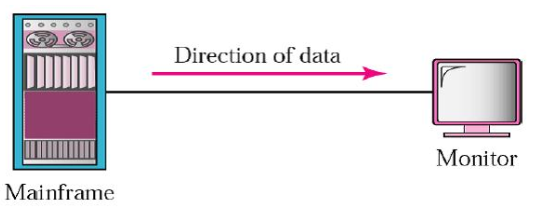
\includegraphics[width=0.80 \textwidth]{./images/simplexx.PNG}}tt
			\end{center}
			\begin{center}
				Figure 1.1 : Reprentation of Simplex data flow.
			\end{center}
			\item \textbf{Half-Duplex : } In half-duplex mode, each of the stations can send and receive the message, but not at the same time. The entire capacity of the channel can be utilized for each direction.
			\begin{center}
				{
\includegraphics[width=0.80 \textwidth]{./images/half-duplex.PNG}}
			\end{center}
			\begin{center}
				Figure 1.2 : Reprentation Half-Duplex data flow.
			\end{center}
			\item \textbf{Full-Duplex : } In full-duplex mode, each stations can transmit and receive simultaneously. The capacity of the channel, however, must be divided between the two directions. A common example of this is telephone network.
			\begin{center}
				{
\includegraphics[width=0.80 \textwidth]{./images/full-duplex.PNG}}
			\end{center}
			\begin{center}
				Figure 1.3 : Reprentation of Full-Duplex data flow.\\\bigskip
			\end{center}
		\end{itemize}
		
		\subsection{Types of Data Communication}
		\begin{flushleft}
			The data communication can be divided into the following types :
			\begin{itemize}
				\item \textbf{Analog Communication : } In analog data communication, the data is sent from one device to another in the form of analog signals or continuous waves. Analog signals are based on a continuous
				electrical wave. Common examples of analog signals are sound waves, light waves or radio waves.
				\item \textbf{Digital Communication : } In digital data communication, the data is sent from one place to another in the form of electrical pulses or digital signals. A digital signal is based on electric pulses. 
				Each electrical pulse represents a stream of bits joined together into bytes. In digital data transmission, data is sent through a telephone line, microwave system, and satellite.\\\bigskip
			\end{itemize}
		\end{flushleft}
		
		\subsection{Model of Communication}
		\begin{flushleft}
			The whole communication process comprise of many small processes that enables the transmission and retrieval of the message signal. A typical communication system consists of various stages of processing of the message signal
			The message, say an audio message, is fed to a transducer to convert the message into an electrical signal. This acts as the input signal and has a low frequency. This input signal is then passed through the transmitter where the signal
			is modulated with the help of a high frequency carrier signal and the modulated signal is transmitted through transmitting antenna into the transmission channel. The modulated signal travels through the channel where some noise
			can affect the transmitted signal. This signal is then catched by the receiver's antenna and demodulation process starts at the receiver end to take out the original message signal from the modulated signal. This signal is then again 
			fed to the transducer to convert the output signal of the demodulator into the original message.
			\begin{center}
				{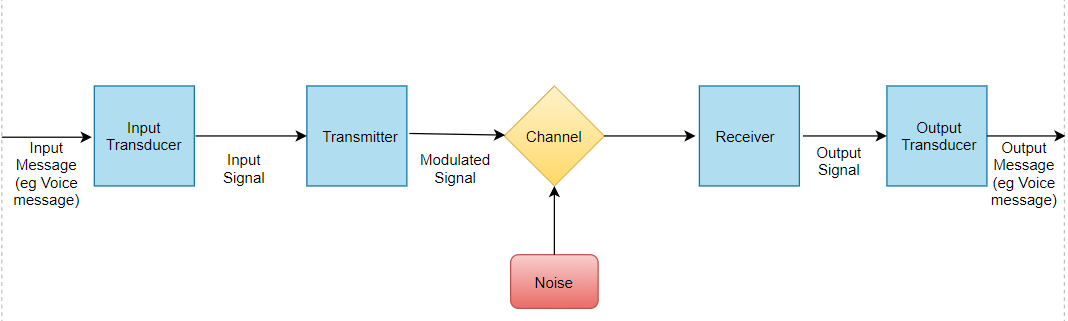
\includegraphics[width=0.80 \textwidth]{./images/modelofcomm.PNG}}
			\end{center}
			\begin{center}
				Figure 1.4 : Schematic reprentation of the model of communication.\\\bigskip
			\end{center}
		\end{flushleft}
		
		\subsection{Modes of Communication}
		\begin{flushleft}
			There are two kinds of modes of communication :
			\begin{itemize}
				\item \textbf{Broadcasting : } In the broadcasting mode of communication there is one sender from which message signals are transmitted to multiple receivers. This kind of communation is unideirectional. A common example of
				bradcasting mode of communication is television network, radio network etc.
				\item \textbf{Point-to-Point Communication : } In the point-to-point mode of communication, the message signal transimited by the sender is received by one receiver. This kind of communications are often bidirectional i.e. both the 
				stations or devices can transmit and receive the message. A common example of point-to-point mode of communication is telephone network.\\\bigskip
			\end{itemize}
		\end{flushleft}
		
		\subsection{Techniques of Communication}
		\begin{flushleft}
			\begin{itemize}
				\item \textbf{Base-Band Communication : } In base-band communication the original message signal is transmitted without modulation into the channel. This kind of communication cannot be employed to long distance communication
				due to the low frequency of the transmitted signal because of which it gets attenuated. Hence, it can be used locally over a small area. It also limits the number of signals that can be
				transmitted through the channel because sending more signals over the channel may lead to interferences of the signals and hence a distorted signal is received at the receiving end.
				\item \textbf{Band-Pass Communication : } In band-pass communication the original low frequency signal is modulated with the help of high frequency carrier signal is then transmitted over the channel. Due to high frequency of
				the transmitted modulated signal, it is less affected by attenuation and can be transmitted over long distances. Band-pass communication enables multiplexing i.e. one channel can be used
				to transmit multiple signals provided all have different frequencies.\\\bigskip
			\end{itemize}
		\end{flushleft}
		
	\end{flushleft}
	\pagebreak
	\section{Modulation}
	\begin{flushleft}
		\subsection{Need of Modulation}
		\begin{flushleft}
			\fontsize{12pt}{18pt}\selectfont
			We must have some strong reasons for why to modulate our message signal as it makes the complete process of communication a bit complex.Here are a few points we need to have a look on :
			\begin{enumerate}
				\item {\large No interference: } Suppose there is a busy channel , where we need to transmit multiple signals , and if the range of frequency is common between any two signal there is a chance of interference among them. During Modulation, the message signal is processed using carrier signals having unique frequencies (carrier frequency) due to which there is no two signals in the channel having same range of frequency and hence the problem of interference is removed.For example , there are 3 signals viz. voice , audio and video whose frequency ranges from 300Hz - 35KHz, 20Hz-20KHz and  0Hz-4.5MHz respectively; being transmitted from the same channel so they are chances of interfering as the range is common.Modulating these signals with 3 different frequencies f1,f2 and f3 woulld help us deal with this.
				
				\item {\large Multiplexing: }The second point is a byproduct of the above advantage. Since, we can have an interference-absent signal transmission for multiple signals through a single channel that is the very idea of multiplexing, which has numerous applications in the field of data communication.Muxing brings along one more advantage of cost reduction.
				
				\item {\large Height Of Antenna: } Signals are actually transmitted and recieved using antennas, which is the most vital part of any bidirectional/unidirectional communication.We can see in the forthcoming sub-topic that height of the antenna could be reduced as a result of modulation.
				
				\item{\large Improves Signal To Noise Ratio: }As the frequency of the modulated signal is very high the chances of noise entry decreases abruptly, due to which the signal to noise improves substantially.
				
				\item{\large Long distance Transmission: }As the frequency increases, the power of signal increases and it does not attenuates easily while a low frequency signal fades out easily and cannot undergo long distance transmissions.
			\end{enumerate}
		\end{flushleft}
		\subsection{Antenna Theory}
		\begin{flushleft}
			\fontsize{12pt}{18pt}\selectfont As we have already talked that,height of the transmitting/receiving antenna depends upon the the signal we are trying to work on.The theory talks about what should be the height of the antenna for a proper transmission; it says that \\\bigskip
			\begin{center}  height of antenna(h) $\propto$ $\frac{wavelength(\lambda)}{4}$
			\end{center}
			we know that,
			\begin{center}
				$\lambda$ = $\frac{c}{f}$                        ,c is the speed of light
			\end{center} 
			From the above famous relation,it is clear that wavelength($\lambda$) varies inversely with frequency(f) of the signal.So the greater the frequency of the transmitting signal the smaller will be the value of $\lambda$ and hence the feasible will be the height of the antenna(h).
			Suppose, we have a signal propagating with a frequency of 15kHz, then wavelength($\lambda$) is given by\\\bigskip
			\begin{center}	$\lambda$= $\frac{3\times 10^8}{15 \times 10^3}$  \\\bigskip
				= 20000 m                  
			\end{center}
			and the height of the antenna is, 
			\begin{center}
				h=$\frac{20000}{4}$    \\\bigskip
				=5000 m
			\end{center}
			which is ofcourse not feasible to build.Hence, the frequency of 10KHz is also falling short for purpose that is why the above mentioned signals have frequencies in the range of MHz.The carrier frequencies in case of modulation have frequencies in this range , which makes it possible to build antennas of practical length.\\\bigskip
			Suppose the frequency of the transmitting signal is 6MHz after modulating ,the wavelength of the signal is :
			\begin{center}
				$\lambda$= $\frac{3\times 10^8}{6 \times 10^6}$  \\\bigskip
				=50m 
			\end{center}
			and now the height of the antenna is,
			\begin{center}
				h=$\frac{50}{4}$     \\\bigskip
				= 12.5 m
			\end{center}
			This time the antenna seems practical to build and hence antenna theory plays a great role in deciding the carrier frequency or indirectly the height of the antennas.
		\end{flushleft}
		\subsection{Modulation Process}
		\begin{flushleft}
			\fontsize{12pt}{18pt}\selectfont
			\begin{enumerate}
				\item  {\large Continuous Wave Modulation(CWM): }The modulated signal in this case is continuous in time domain.It is further divided into : \\\bigskip
				\begin{itemize}
					\item {\fontsize{14pt}{20pt}\selectfont Amplitude Modulation(AM): } The amplitude of the carrier signal varies in accordance with the input baseband signal.Different types of AM are : \\\bigskip
					\begin{enumerate}
						\item \textbf{Double sideband Full Carrier(DSB-FC) }:The transmission of a modulated signal which contains a carrier along with sidebands is termed as DSB-FC.
						
						\item \textbf{Double sideband Suppressed carrier(DSB-SC) }: The above discussed transmission is known to be inefficient as two-third of the total power in the carrier wave is being wasted having no information.If we suppress the above type of signals and the power that is saved is distributed among the two sidebands we get DSB-SC.
						
						\item \textbf{ Single sideband Suppressed carrier(SSB-SC) }: As both the sidebands are  carrying same information two times, its better if we suppress one of the two. The suppression of one of them along with the carrier wave and transmitting a single sideband is what we call Single sideband Suppressed carrier system or SSB-SC.It has high power as compared to DSB-FC/DSB-SC.
						
						\item \textbf{Vestige sideband Suppressed carrier(VSB-SC) }: As transmission of two sidebands is unnecassary , but transmitting single sideband leads to loss of information.So in vestigial modulation a part of signal(vestige) is modulated along with each sideband.In other words, a part of upper side band is also transmitted with lower sideband.To avoid interferences, a guard band having very small width is also laid along with each sidebands.
						VSB modulations are highly efficient and filter design is quite easy as high accuracy is not demanded.The only point where it lacks is demodulation becomes a difficult task in this kind of modulations.
						
						\item \textbf{Independent sideband Suppressed carrier(ISB-SC) }:Input signal is modulated by two different modulating signals.Here the transmitter comprises of two independent SSB-SC modulators. one of the modulator generates the upper sideband and the other generates the lower sideband.The output signals from the two modulators are combined to form a DSB ,where the sidebands are completely independent but are symmetrical about a common carrier freqeuncy.  \\\bigskip
					\end{enumerate}
					\item {\fontsize{14pt}{20pt}\selectfont Angle Modulation : }It has been further divided into two parts :
					\begin{enumerate}
						\item \textit{Frequency Modulation }: In this case,the carrier wave frequency is varied according to the modulating signal whereas the amplitude remains constant.Two types of FM are explained below :
						\begin{enumerate}
							
							\item \textbf{Narrow Band FM : }As the name suggests,it is the FM wave with comparitively small bandwith.The modulation index is as small as 1 radian.\\\smallskip
							Its uses are in the fields of FM mobile communications like ambulances,taxies,etc.  
							
							\item \textbf{Wide Band FM : }FM waves having infinitely large frequency comes under this category.It ideally contains the carrier wave and an infinite number of sidebands located symmetrically around it.\\\smallskip
							Its widely applied in th fields of Television,FM radio,etc.
						\end{enumerate}
						\item \textit{Phase Modulation }: The variation of the phase of carrier wave linearly in accordance with the input signal is phase modulation.It is of two types :
						\begin{enumerate}
							\item \textbf{Narrow Band Phase Modulation }
							\item \textbf{Wide Band Phase Modulation }
						\end{enumerate}		        		
					\end{enumerate}
				\end{itemize}
				\item  {\large Pulse Modulation(PM): }In this kind of modulation,some parameter of a pulse train is varied in accordance with the input message signal.It is mainly divided in two parts :
				\begin{itemize}
					\item {\fontsize{14pt}{20pt}\selectfont Analog Pulse Modulation(APM): }
					\begin{enumerate}
						\item \textbf{Amplitude PM  }
						
						\item \textbf{Position PM  }
						
						\item \textbf{Phase PM  }
					\end{enumerate}
					
					\item {\fontsize{14pt}{20pt}\selectfont Digital Pulse Modulation(DPM): }
					\begin{enumerate}
						\item \textbf{Baseband : }
						\begin{itemize}
							\item Pulse Code Modulation(PCM)
							\item Differential Pulse Code Modulation(D-PCM)
							\item Delta Modulation
							\item Adaptive Delta Modulation
						\end{itemize}
						\item \textbf{Bandpass : }
						\begin{itemize}
							\item Binary
							\item M-ary
						\end{itemize}
					\end{enumerate}
				\end{itemize}
			\end{enumerate}
		\end{flushleft}
	\end{flushleft}
	\pagebreak
	\section{Amplitude Modulation(AM)}
	\begin{flushleft}
		\subsection{Introduction}
		\begin{flushleft}
			Amplitude Modulation is a modulation technique in which the amplitude of another signal called \textit{carrier signal} $c(t)$ is varied in accordance with the \textit{message/input/modulating signal} $m(t)$. The modulating signal or $m(t)$ contains the intended message or information that is to be transmitted across the channel. The modulating signal contains the intended message or information sometimes consisting of audio data, as for an example in \textit{AM} radio broadcasting, or two-way radio communications.
		\end{flushleft}
		\subsection{Modulation Process}
		\begin{flushleft}
			The high-frequency sinusoidal waveform(i,e., \textit{carrier signal}) is modulated with respect to the input signal by combining it with the message signal using a \textit{multiplier} or \textit{mixer}. It is worth mentioning that mixing is a non-linear operation because it generates new frequencies. An example of visual realization of Amplitude modulation is shown as follows:
			\begin{center}
				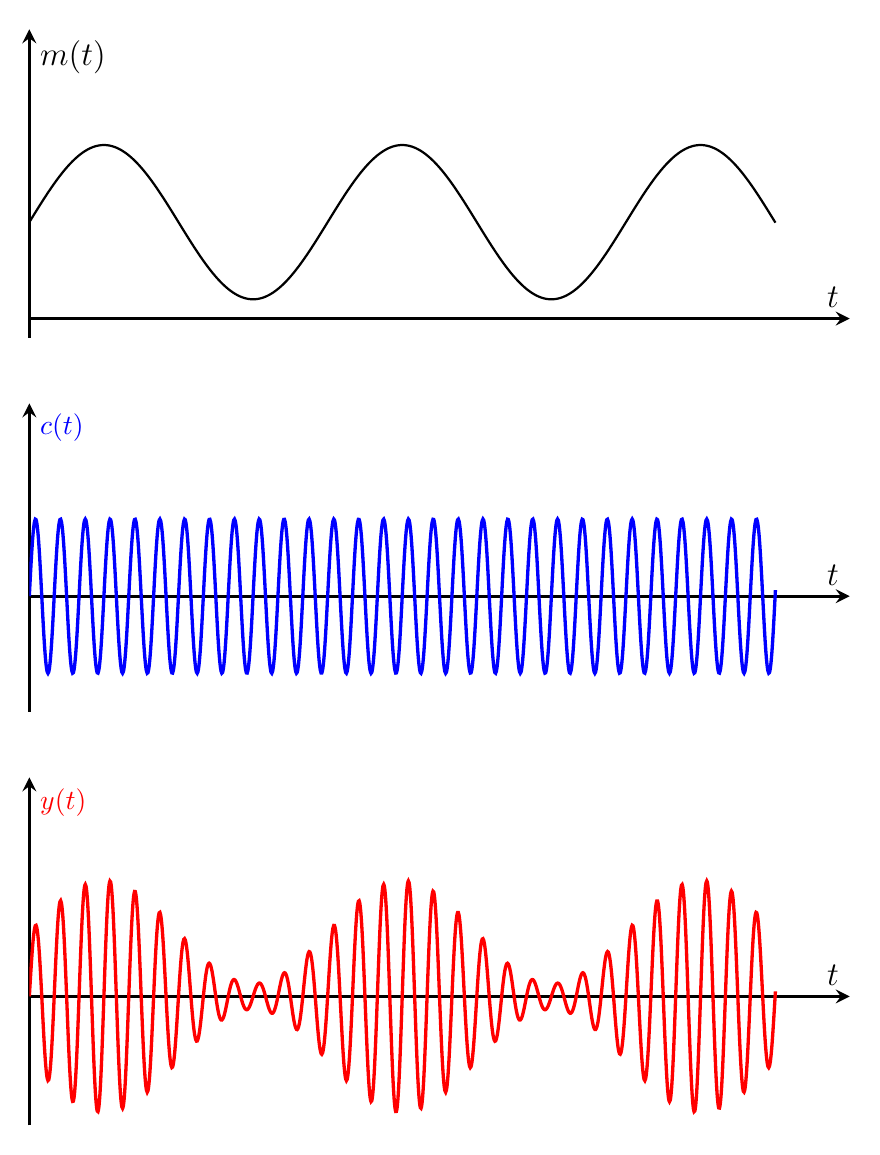
\begin{tikzpicture}[samples=1000, domain=0:10*pi]
				
				\begin{axis}[
				width=12cm, height=5.5cm,
				xtick=\empty,
				ytick=\empty,
				xlabel={\large $t$},
				ylabel={\large $m(t)$},
				xmin=0, xmax=11*pi,
				ymin=-0.5, ymax=7.5,
				axis lines = middle,
				very thick,
				trig format = rad
				]
				\addplot [no markers, smooth, thick] {2.5 + 2*sin(0.5*x)};
				\end{axis}
				
				\begin{axis}[
				at={(0, -4.75cm)},
				width=12cm, height=5.5cm,
				xtick=\empty,
				ytick=\empty,
				xlabel={\large $t$},
				ylabel={\textcolor{blue}{$c(t)$}},
				xmin=0, xmax=11*pi,
				ymin=-3, ymax=5,
				axis lines = middle,
				very thick,
				trig format = rad
				]
				\addplot [no markers, smooth, blue, very thick] {2*sin(6*x)};
				\end{axis}
				
				\begin{axis}[
				at={(0, -10cm)},
				width=12cm, height=6cm,
				xtick=\empty,
				ytick=\empty,
				xlabel={\large $t$},
				ylabel={\textcolor{red}{$y(t)$}},
				xmin=0, xmax=11*pi,
				ymin=-10, ymax=17,
				axis lines = middle,
				very thick,
				trig format = rad
				]
				\addplot [no markers, smooth, red, very thick] {(2.5 + 2*sin(0.5*x)) * 2*sin(6*x)};
				\end{axis}
				\end{tikzpicture}
			\end{center}
			\begin{center}
				The signal in red \textit{i.e.,} $y(t)$ is the \textit{amplitude modulated} wave.
			\end{center}
		Generally we have the modulated signal as $y(t)=m(t).c(t)$, but in case of amplitude modulation if we use this form, there is a serious problem of phase reversal \textit{i.e.,} the signal crosses the $x-axis$, which in turn when multiplication causes the problem of phase reversals.
		\end{flushleft}
		\begin{center}
			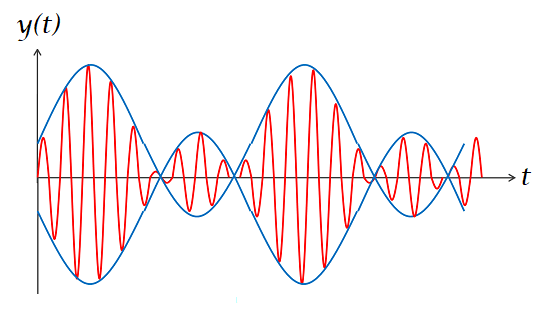
\includegraphics[width=0.60 \textwidth]{./images/SDC-Phase Reversal_1.png}
		\end{center}
		The mechanism of retrieval of original message signal from such a phase reversed signal is complicated and impractical for implementation. So, we improvise and solve this problem.\\\smallskip
		To do so, we shift our message signal $m(t)$, by some \textit{DC} value say $A$ and then multiply it with its carrier signal, for modulation purposes.\\\smallskip
		The general form of such signal is given by the following equation,
		\begin{equation}
			y(t)=A_c [1+k_a m(t)]cos(2 \pi f_c t)
		\end{equation}
		From the above equation if we observe then, the message signal is measured in $volts$. Therefore, by dimensional analysis the unit of $k_a$ is $volts^{-1}$.So,\\\smallskip
		$k_a$, is the amplitude sensitivity.\\
		$m(t)$ is the message/modulating signal.\\
		$y(t)$ is the modulated wave.\\\smallskip
		The \textit{envelope} of $y(t)$ in particular has same shape as the baseband signal $m(t)$ provided that the following two requirements are satisfied,
		\begin{itemize}
			\item{
				The amplitude of $k_a m(t)$ represented as $|k_a m(t)|$ is always less than unity,\textit{i.e.,}
				\begin{equation}
					|k_a m(t)| \leq 1,\enspace \forall \enspace t
				\end{equation}
				\begin{itemize}
					\item{It ensures that the function $1+k_a m(t)>0$, and since an envelope is positive. We can represent it as $A_c [1+k_a m(t)]$.}
					\item{When, $|k_a m(t)|>1$, $y(t)$ becomes overmodulated, resulting in carrier phase reversals whenever the factor as mentioned $1+k_a m(t)$ crosses zero.
					\item{The absolute maximum value of $k_a m(t)$ multiplied by $100$ is referred to as \textit{percentage modulation}}}
				\end{itemize}
			}
			\item{
				The carrier frequency $f_c$ is much greater than the highest frequency component $W$ of the message signal $m(t)$\textit{i.e.,}
				\begin{equation}
					f_c \gg W
				\end{equation}
				\begin{itemize}
					\item{If the above condition is not satisfied, an envelope cannot be realized successfully. The component $W$, is called the message bandwidth.}
				\end{itemize}
			}
		\end{itemize}
		
		If we take the \textit{fourier} transform of \textit{equation} (), then we have,
		
		\begin{center}
		$$F(y(t))=Y(f)=\int_{-\infty}^{\infty} A_c [1+k_a m(t)]cos(2 \pi f_c t) dt$$\\\smallskip
			\begin{flushleft}
				Upon, using the following results we simplify the above equation,\\\smallskip
			\end{flushleft}
			\begin{itemize}
				\item{$cos(x)=\dfrac{e^x-e^{-x}}{2}$}
				\item{$\int_{-\infty}^{\infty} e^{j 2 \pi f (t-a)} df=\delta (t-a)=\delta (a-t)$}
			\end{itemize}
			
		\end{center}
		We find that,
		\begin{equation}
			F(cos(2 \pi f_c t))=\dfrac{\delta(f-f_c)+\delta(f+f_c)}{2}
		\end{equation}
		\textit{equation} $Y(f)$ implies,
		\begin{equation}
		Y(f)=\dfrac{A_c}{2}[\delta(f+f_c)+\delta(f-f_c)]+\dfrac{k_a A_c}{2}[M(f+f_c)+M(f-f_c)]
		\end{equation}
		\begin{center}
			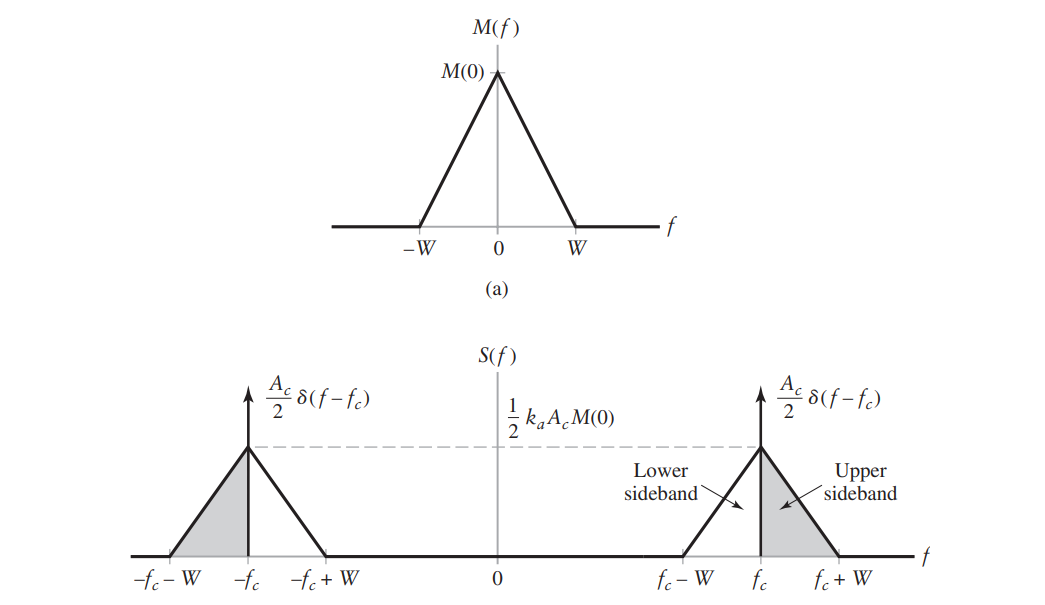
\includegraphics[width=0.99 \textwidth]{./images/AM modulation_1.png}
		\end{center}
		\begin{center}
			The above figure represents all the signals given by \textit{equation} $5$. Figure (a) in above gives the frequency spectrum of signal $m(t)$
		\end{center}
		\pagebreak
		\begin{flushleft}
			We now analyze the spectrum given by the above figure.
			\begin{itemize}
				\item{The frequency of the carrier signal should be sufficiently higher than that of the modulating signal \textit{i.e.,} the condition given by the \textit{equation} (3) should hold. Otherwise, both the side bands will interfere each other.}
				\item{The frequency above $f_c$ is known as upper sideband, below $f_c$ is referred to as the lower sideband. For negative frequencies: The upper sideband is below $-f_c$ as shaded region shows clearly and the lower sideband is above $-f_c$. The condition $f_c>W$ ensures that the sidebands do not overlap, in accordance with point above.}
				\item{For positive frequencies, the highest frequency component of the AM wave equals $f_c + W$, and the lowest frequency component equals $f_c-W$. The difference between these two frequencies defines the \textit{transmission bandwidth} $B_T$ for an AM wave.}
				\begin{equation}
					B_T = 2W
				\end{equation}
			\end{itemize}
		\end{flushleft}
	
		\subsection{Single Tone Modulation}
		\begin{flushleft}
			In this form of Amplitude Modulation both message and carrier waves are sinusoidal signals. We will do a brief mathematical analysis of the same,\\\smallskip
			We will consider the message signal and the carrier signal as follows:\\\smallskip
			\begin{equation}
			m(t)=A_m cos(2 \pi f_m t)
			\end{equation}
			\begin{equation}
			c(t)=A_c cos(2 \pi f_c t)
			\end{equation}
			The modulated signal will be,
			\begin{equation}
			y(t)=A_c [1+\mu cos(2 \pi f_m t)] cos(2 \pi f_c t)
			\end{equation}
			where, $\mu = k_a A_m$, and to avoid overmodulation $\mu$ should be kept relatively small \textit{i.e.,} $|\mu|<1$.\\\smallskip
			If $A_{max}$ and $A_{min}$ represents the maximum and minimum values of the the envelope of the modulated wave then we have,
			\begin{equation}
			\dfrac{A_{max}}{A_{min}}=\dfrac{A_c (1+\mu)}{A_c (1-\mu)}
			\end{equation}
			\begin{center}
				$\mu =\dfrac{A_{max} - A_{min}}{A_{max} + A_{min}}$
			\end{center}
			We have another useful relation for finding the modulation factor $\mu$.\\\smallskip
			Using the following formula, and using it in \textit{equation} (9) we have,
			\begin{center}
				$y(t)=A_c cos(2 \pi f_c t) + \dfrac{1}{2} \mu A_c cos[2 \pi (f_c +f_m)t]+ \dfrac{1}{2} \mu A_c cos[2 \pi (f_c -f_m)t]$
			\end{center}
			Taking the Fourier Transform of the above equation we have,
			\begin{equation}
				Y(f)=\dfrac{1}{2} A_c [\delta (f - f_c) + \delta(f+f_c)] + \dfrac{1}{4} \mu A_c cos[\delta (f - (f_c+f_m)) + \delta (f + (f_c+f_m))]+ \dfrac{1}{4} \mu A_c cos[\delta (f - (f_c-f_m)) + \delta (f + (f_c-f_m))]
			\end{equation}
			\begin{center}
				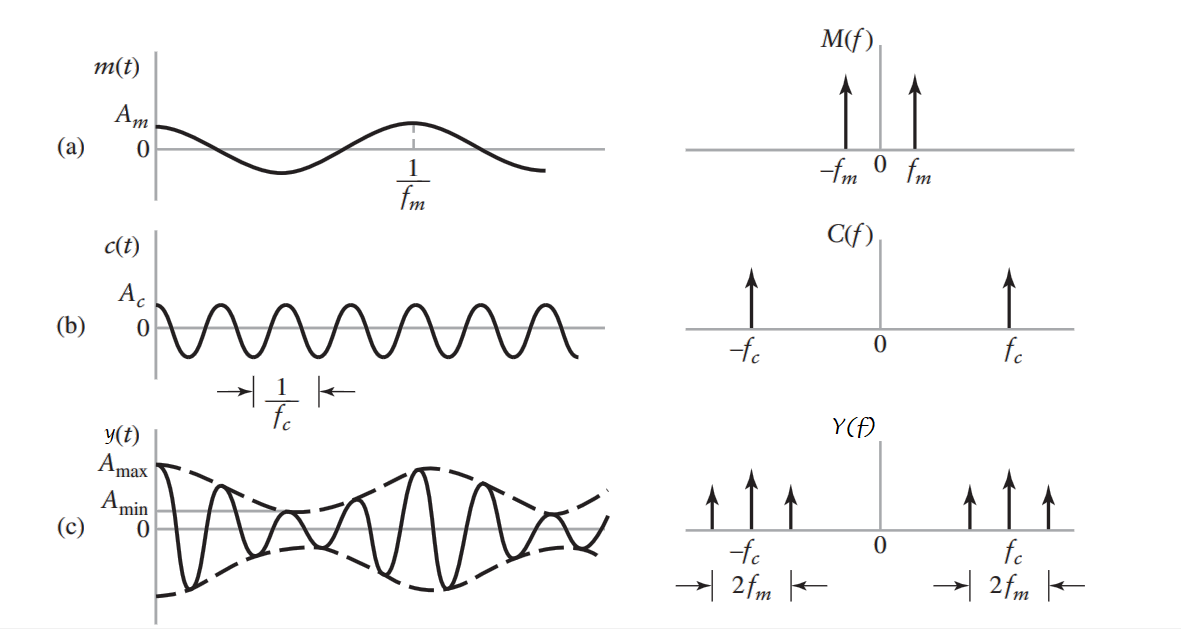
\includegraphics[width=0.99 \textwidth]{./images/Single tone.png}
			\end{center}
			The above diagram represents the actual time varying signal together with it frequency spectrum on the right.\\\smallskip
			\subsubsection{Power of Single Tone Modulated Signal}
			\begin{flushleft}
				The power of single tone modulated signal is given by,
				\begin{center}
					$P_{total}=P_{carrier}+P_{USB}+P_{LSB}$\\\bigskip
					where LSB stands for Lower Side Band and USB for Upper Side Band, in general Power $P$ is given by,\\\bigskip
					$P=\dfrac{V_{rms}^{2}}{R}$
					where, $R$ is the resistance of the antenna,\\\bigskip
					If $R=1$ then we have,\\\bigskip
					Carrier power $P_{carrier}=\dfrac{1}{2} A_c^2$\\\bigskip
					Carrier power $P_{LSB}=\dfrac{1}{8} \mu^2 A_c^2$\\\bigskip
					Carrier power $P_{USB}=\dfrac{1}{8} \mu^2 A_c^2$\\\bigskip
					Total Power $P_{total}=P_{carrier}[1+\dfrac{\mu^2}{2}]$
				\end{center}
			In particular the ratio of total power in the sideband to the total power in the modulated wave is equal to,\\\bigskip
			\begin{equation}
				\dfrac{\mu^2}{2+\mu^2}
			\end{equation}
			From the above factor we can see that the ratio,
			\begin{itemize}
				\item{Depends only on the modulation factor $\mu$}
				\item{If $\mu = 1$, the total power in the two side frequencies of the resulting AM wave is only one-third of the total power in the modulated wave.}
				\item{If the percentage modulation is less than 20\%, the power in one side frequency is less than 1\% of the total power of the Amplitude modulated wave. }
			\end{itemize}
			\end{flushleft}
			\subsubsection{Power of Multi Tone modulated signal}
			\begin{flushleft}
				Generalzing the the \textit{equation} (12) for multi-tone signal we have,
				\begin{equation}
				\dfrac{\mu_{mt}^2}{2+\mu_{mt}^2}
				\end{equation}
				Where, $\mu_{mt}^{2}=\sum\limits_{i=1}^n \mu_{i}^{2}$, here $\mu_i$'s are the modulation factor of the individual message signal.
				
			\end{flushleft}
		\end{flushleft}
	
		\subsection{Generation of Amplitude Modulated Wave}
		\begin{flushleft}
			The block diagram of the square law modulator is shown as follows,\\
			\begin{center}
				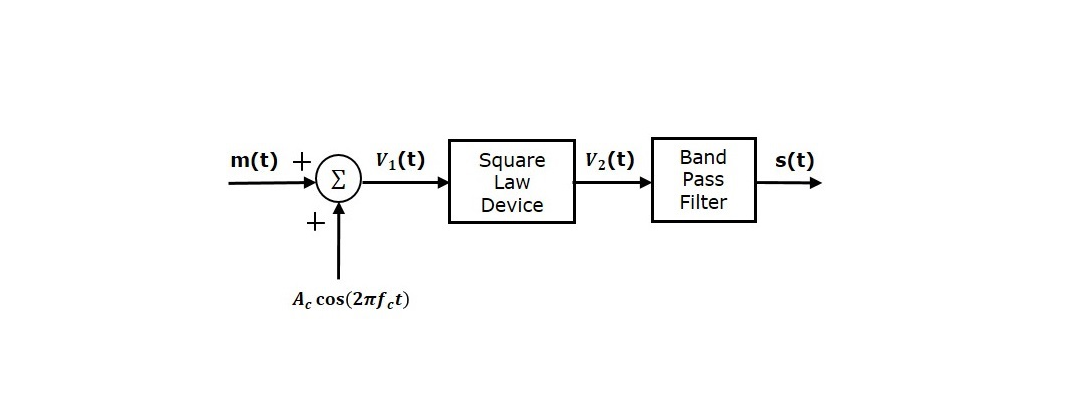
\includegraphics[width=0.99 \textwidth]{./images/Square Law modulator.png}
			\end{center}
			If our modulating signal is $m(t)$ and carrier signal is $c(t)=A_c cos(2 \pi f_c t)$.\\
			\begin{center}
				$V_1 (t) = m(t) + A_c cos(2 \pi f_c t) $
			\end{center}
			If the signal $V_1 (t)$ is applied as an input to a nonlinear device like diode. The characteristics of the diode are closely related to square law, the equation of which can be represented as,
			\begin{equation}
				V_2 (t) = k_1 V_1 (t) + k_2 V_1 ^ {2} (t)
			\end{equation}
			where, $k_1$ and $k_2$ are constants.\\
			Substituting $V_1 (t) $ in \textit{equation} (14) we have,
			\begin{equation}
				V_2 (t) = k_1 [m(t) + A_c cos(2 \pi f_c t)] + k_2 [m(t) + A_c cos(2 \pi f_c t)] ^ {2} (t)
			\end{equation}
			Simplifying $V_2 (t)$ we have,
			\begin{equation}
				V_2 (t) = k_1 m(t) + k_2 m^2 (t) + k_2 A_c ^ 2 cos^2 (2 \pi f_c t) + k_1 A_c [1+(\dfrac{2 k_2}{k_1})] cos(2 \pi f_c t)
			\end{equation}
			The first \textit{three} terms in the above equation are unwanted and only the last term was wanted signal, so we can remove the first three terms by passing the above signal \textit{i.e.,} $V_2 (t)$ through a band pass filter. Therefore, the final output of the square law modulator is,
			\begin{equation}
				y(t) = k_1 A_c [1+(\dfrac{2 k_2}{k_1})] cos(2 \pi f_c t)
			\end{equation}
			comparing the above equation with the standard equation of the amplitude modulated wave in \textit{equation} (1) we see that it is indeed the required amplitude modulated wave.
		\end{flushleft}
		
		\subsection{Types of Amplitude Modulation}
		\begin{flushleft}
			\begin{itemize}
				\item{\textbf{Double Side Band - with Carrier(DSB-WC)} : This form of Amplitude Modulation is most widely used. All radio channels in the AM band use this type of modulation.}
				\item{\textbf{Double Side Band - Suppressed Carrier(DSB-SC)} : This form of Amplitude Modulation is same as the above mentioned except for the fact that it is without carrier(\textit{suppressed}).}
				\item{\textbf{Single Side Band (SSB)} : In this form of AM the only half of the signal of DSB-SC is used.}
				\item{\textbf{Vestigial Side Band (VSB)} : This is the modified version of SSB, to ease the generation and reception of the signal.}
			\end{itemize}
		\end{flushleft}
		\subsection{Advantages}
		\begin{itemize}
			\item{It is simple to implement}
			\item{It can be demodulated using a circuit consisting of very few
				components
}
			\item{AM receivers are inexpensive because no specialized components
				are required}
		\end{itemize}
		\subsection{Disadvantages}
		\begin{itemize}
			\item{It is not efficient with respect to power usage}
			\item{It is not efficient in bandwidth; requires a bandwidth equal to twice the highest audio frequency
}
			\item{It is prone to high levels of noise because most noise is amplitude based and AM detectors are sensitive to it.}
		\end{itemize}
	\end{flushleft}
	\pagebreak
	\section{Frequency Modulation}
	\begin{flushleft}
	The angle modulation in which the instantaneous frequency $f_i(t)$ of the carrier signal is varied linearly with the message signal is called frequency modulation.Mathematically, if $m(t)$ be the message signal(voltage waveform) and $f_c$ be the frequency of the unmodulated carrier  signal then 
	\begin{equation} \label{eq:erl}
	f_i(t)=f_c+k_fm(t)
	\end{equation}
	where $k_f$ is the frequency-sensitivity factor of the modulator(in hertz per volt)
	\subsection{Time Equation for Frequency Modulated Wave}
	Let $\theta_i(t)$ denote the angle of a modulated sinusoidal carrier at time t and the resulting angle-modulated wave is 
	\begin{equation} \label{eq:erl}
	s(t)=A_c \cos{[\theta_i(t)]}
	\end{equation}
	where $A_c$ is the carrier amplitude.\\
	If $f_i(t)$ be the instantaneous frequency of resulting FM wave then 
	\begin{equation} \label{eq:erl}
	\displaystyle{f_i(t)= \frac{1}{2\pi}\frac{d\theta_i(t)}{dt}}
	\end{equation}
	Integrating Eq (3) with respect to time, we get
	
	
			$$\theta_i(t)= 2\pi \int_0^tf_i(\tau)\,d\tau=2\pi f_ct+2\pi k_f \int_0^tm(\tau)\,d\tau$$
			
	%$$\theta_i(t)= 2\pi \int_0^tf_i(\tau)\,d\tau$=2\pi f_ct+2\pi k_f \int_0^tm(\tau)\,d\tau$$
	\begin{flushleft}
		where the second term accounts for the increase or decrease in the instantaneous phase due to the message signal $m(t)$.\\
		Therefore, the frequency modulated wave is given by
	\end{flushleft}
	$$s(t)=A_c \cos{[2\pi f_ct+2\pi k_f \int_0^tm(\tau)\,d\tau]}$$ 
	\subsection{Narrow Band Frequency Modulation}
	Consider a sinusoidal modulating wave defined by
	$$m(t)= A_m \cos{2\pi f_m t}$$
	Then instantaneous frequency of the resulting FM wave is
	%%NILAM CHECK THIS-> I have changes
	\begin{center} \label{eq:erl}
	$f_i(t)=f_c+k_f A_m \cos{2\pi f_m t}$\\
	$=f_c+\Delta f \cos{2\pi f_m t}$
	\end{center}
	where $\Delta f= k_f A_m $ is called the frequency deviation which represents the maximum departure of the instantaneous frequency of the FM wave from the carrier frequency.\\
	The angle $\theta_i(t)$ of the FM wave is given by
	$$\theta_i(t)=2\pi f_ct+2\pi k_f \int_0^tA_m \cos{2\pi f_m t} \,d\tau$$
	Or             $$\theta_i(t)=2\pi f_ct+\frac{\Delta f}{f_m} \sin{2 \pi f_m t}$$
	Or             $$\theta_i(t)=2\pi f_ct+\beta \sin{2 \pi f_m t}$$
	where $\displaystyle{\beta=\frac{\Delta f}{f_m}}$ is called
	the modulation index of the FM wave( measured in radians).
	
	The resulting FM wave is 
	\begin{equation}
	s(t)=A_c \cos{[2\pi f_ct+\beta \sin{2 \pi f_m t}]}
	\end{equation}
	Or
	$$s(t)=A_c \cos{[2\pi f_ct]}\cos{[\beta \sin{2 \pi f_m t}]}-A_c \sin{[2\pi f_ct]}\sin{[\beta \sin{2 \pi f_m t}]}  $$
	For NBFM the modulation index is small compared to one radian.So we can assume 
	$$\cos{[\beta \sin{2 \pi f_m t}]}=1$$
	and $$\sin{[\beta \sin{2 \pi f_m t}]}=\beta \sin{2 \pi f_m t}$$
	Then the narrow band frequency modulated signal is 
	\begin{equation}
	s(t)= A_c \cos{[2\pi f_ct]}- \beta A_c\sin{[2 \pi f_c t]} \sin{[2 \pi f_m t]}
	\end{equation}
	\begin{figure}
		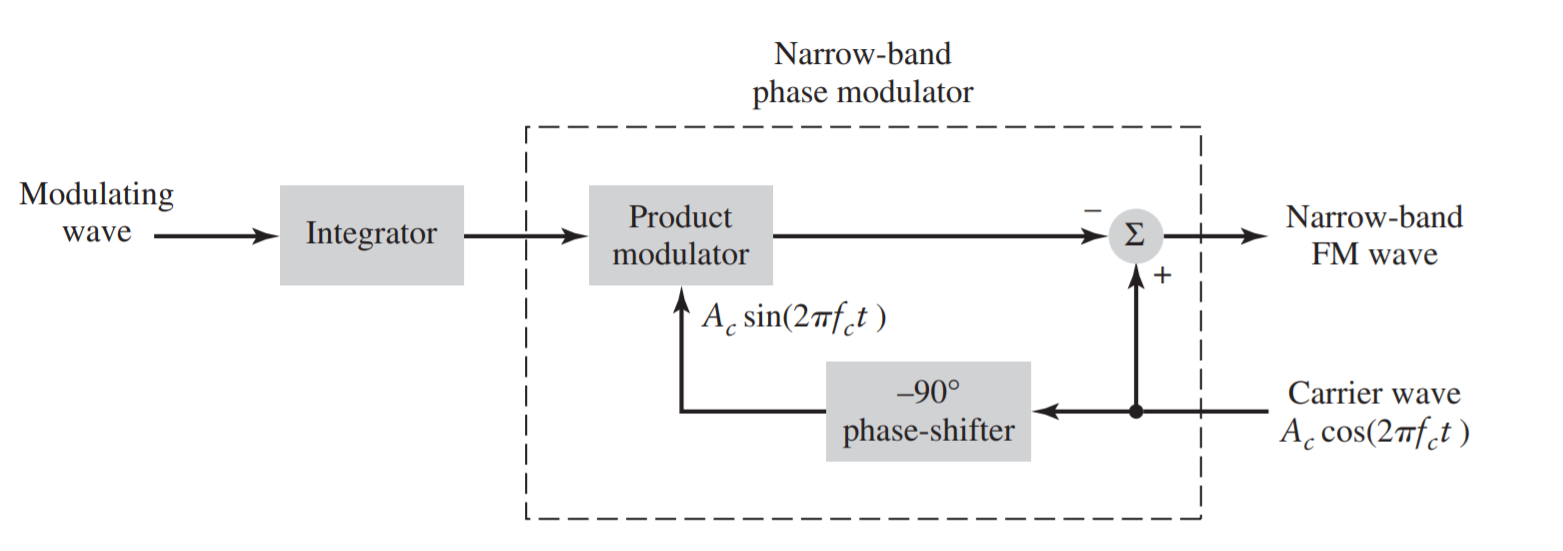
\includegraphics[scale=0.4]{./images/BD1.png}
		\caption{Block diagram of an indirect method for generating a narrow-band FM wave.}
		\label{BD1}
	\end{figure}
	A block diagram is shown above of generating NBFM signal. This modulator involves splitting the carrier wave $A_c\cos{2\pi f_c t}$ into two paths. One path is direct and the other path contains a degree phase-shifting network and a product modulator, the combination of which generates a DSB-SC modulated wave. The difference between these two signals produces a narrow-band FM wave.
	
	\subsection{Wide Band Frequency Modulation}
	The frequency modulated signal for which modulation index $\beta$ is greater than 1 is called wide band frequency modulated signal.\\
	The time equation for WBFM signal can be written with the help of Bessel function. The wide band frequency modulated signal $s(t)$ can be written as 
	\begin{equation}
	s(t)= A_c \sum \limits_{n=-\infty}^\infty J_n(\beta) \cos{[2\pi(f_c+nf_m)t]}
	\end{equation}
	The discrete spectrum of $s(t)$ is obtained by taking the Fourier transforms of both sides of Eq (7) as below
	\begin{equation}
	S(f)= \frac{A_c}{2} \sum \limits_{n=-\infty}^\infty J_n(\beta)[ \delta(f-f_c-nf_m)+\delta(f+f_c+nf_m) ]
	\end{equation}
	where $S(f)$ is Fourier Transform of $s(t)$. The above equation shows that the spectrum of $S(f)$ consists of an infinite number of delta functions spaced at $f=f_c\pm nf_m$ for n=0,1,2,$\cdots$
	\subsubsection{Power of a WBFM signal}
	The average power of an WBFM wave can be determined from
	\begin{equation}
	P_t= \sum \limits_{n=-\infty}^\infty \frac{[{A_cJ_n(\beta)}]^2}{2}
	\end{equation}
	which can be simplified using the property
	$$\sum \limits_{n=-\infty}^\infty J_n(\beta)^2=1$$
	The simplified average power of WBFM signal is
	\begin{equation}
	P_t= \frac{A_c^2}{2}
	\end{equation}
	
	\subsection{Carson's Rule}
	In theory, an FM wave contains an infinite number of side-frequencies so that the bandwidth required to transmit such a modulated wave is similarly infinite in extent.But in practice, the FM wave is effectively limited to a finite number of significant side-frequencies compatible with a specified amount of distortion.
	Let us consider first the case of an FM wave generated by a single-tone modulating wave of frequency $f_m$. In such an FM wave, the side-frequencies that are separated from the carrier frequency $f_c$ by an amount greater than the frequency deviation $\Delta f$ decrease rapidly toward zero, so that the bandwidth always exceeds the total frequency excursion, but nevertheless is limited. Specifically, we may identify two limiting cases: \\
	1. For large values of the modulation index $\beta$the bandwidth approaches, and is only slightly greater than the total frequency excursion $2\Delta f$\\
	2. For small values of the modulation index $\beta$ the spectrum of the FM wave is effectively limited to the carrier frequency $f_c$ and one pair of side-frequencies at$f_c\pm f_m$ so that the bandwidth approaches$2f_m$\\
	Thus, the transmission bandwidth of an FM wave generated by a single-tone modulating wave of frequency $f_m$ is defined by
	$$B_T=2\Delta f +2f_m=2\Delta f(1+\frac{1}{\beta}) $$
	This is called Carson's rule.
	
	
	\subsection{Generation of FM Waves}
	There are two methods of generating frequency modulated waves, the first one is direct and the other indirect method.
	\subsubsection{Direct Method}
	The direct method uses a sinusoidal oscillator, with one of the reactive elements (like capacitive element) in the tank circuit of the oscillator being directly controllable by the message signal. It is capable of providing large frequency deviations. But a serious limitation of the direct method is the tendency for the carrier frequency to drift, which is usually unacceptable for commercial radio applications.\\
	To overcome this limitation, frequency
	stabilization of the FM generator is required, which is realized through the use of feedback around the oscillator.
	Although the oscillator may be simple to build, the use of frequency stabilization adds system complexity to the design of the frequency modulator.
	
	\subsubsection{Indirect Method:Armstrong Modulator}
	\begin{center}
		\begin{figure}[!ht]
			\centering
			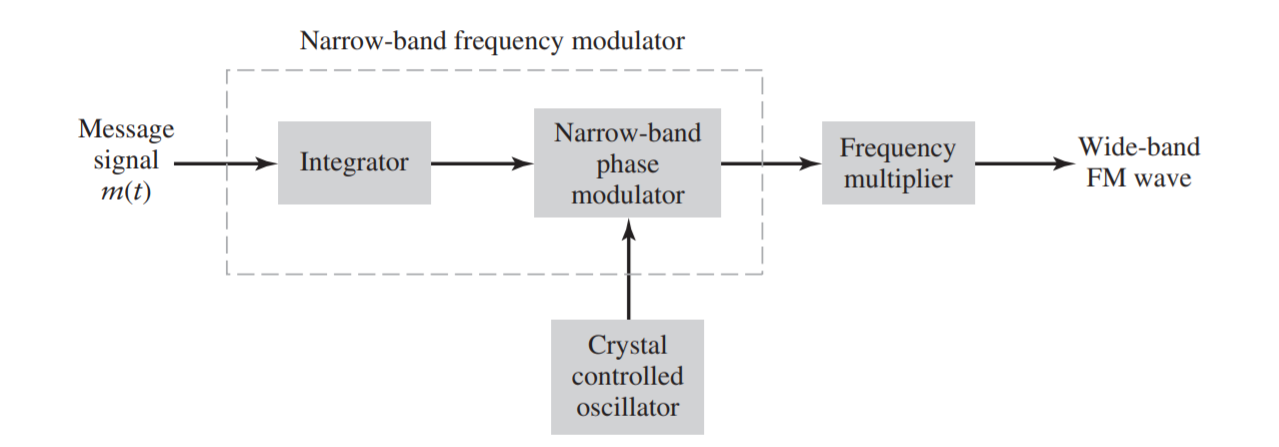
\includegraphics[scale=0.4]{./images/BD2.png}
			\caption{Block diagram of an indirect method for generating a narrow-band FM wave.}
			\label{BD2}
		\end{figure}
	\end{center}
	
	
	A simplified block diagram of this indirect FM system is shown in below fig. The message signal $m(t)$ is first integrated and then used to phase-modulate a crystal-controlled oscillator which provides frequency stability. In order to minimize the distortion inherent in the phase modulator, the maximum phase deviation or modulation index is purposely kept small, thereby resulting in a narrow-band FM wave. The narrow band FM wave is next multiplied in frequency by means of a frequency multiplier so as to produce the desired wide-band FM wave.
	\end{flushleft}
	\pagebreak
	\section{Experimentation}
	\pagebreak
	\section{Simulation}
	\pagebreak
	\section{Code}
	\pagebreak
	\section{Attenuation}
	\begin{flushleft}
		
		\subsection{Definition} 
		\begin{flushleft}
		When a digital or analog signal travels through a medium it loses some of its energy so that it can overcome the resistance of the medium. This loss of energy is called attenuation.That is why a wire carrying electrical signals gets warm. Some of the electrical energy of the signal is converted into heat. To compensate for this loss, amplifiers are used to amplify the signal.Signal amplification electrically increasing the strength of a line signal by one of several technical methods. Typically, on computer networks, amplification includes logic for noise reduction to prevent the underlying message data from becoming corrupted in the process.
		
		\end{flushleft}
		
		\begin{center}
			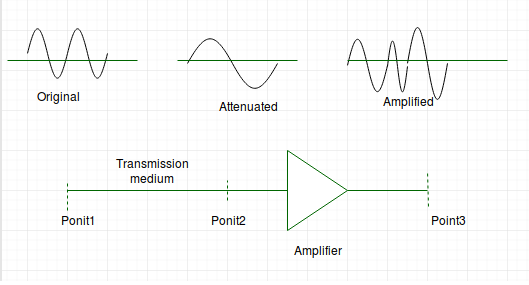
\includegraphics[width=0.80 \textwidth]{./images/NKK1.png}
		\end{center}
		\begin{center}
			Figure: Effect of Attenuation and Amplification
		\end{center}
		
		\subsection{How to measure attenuation} 
		\begin{flushleft}
		The extent of attenuation is expressed in decibels (dBs).If $P_s$ is the signal power at the transmitting end (source) of a communications circuit and $P_d$ is the signal power at the receiving end (destination), then $P_s\, >\, P_d$. The power attenuation $A_p$ in decibels is given by the formula:
		$$A_p= 10\log_{10}{\frac{P_s}{P_d}}$$
		Attenuation can also be expressed in terms of voltage. If $A_v$ is the voltage attenuation in decibels, $V_s$ is the source signal voltage, and $V_d$ is the destination signal voltage, then:$$A_v= 20\log_{10}{\frac{V_s}{V_d}}$$\\\bigskip
		\item Importance of Determination of Attenuation
		\paragraph{}
		Attenuation is important in telecommunications and ultrasound applications because it’s critical to determine signal strength as a function of distance. Minimizing the loss of attenuation is important in microwave, wireless and cellular applications because to function correctly an optical data link depends on modulated light reaching the receiver with enough power to be correctly demodulated. This power is reduced through attenuation, resulting in a loss of the light signal that’s being transmitted.
		\end{flushleft}
		\subsection{ Causes of attenuation} 
		\begin{flushleft}
		Attenuation can relate to both hard-wired connections and to wireless transmissions. There are many instances of attenuation in telecommunications and digital network circuitry. Inherent attenuation can be caused by a number of signaling issues including:\\\bigskip
		1. Transmission medium - All electrical signals transmitted down electrical conductors cause an electromagnetic field around the transmission. This field causes energy loss down the cable and gets worse depending upon the frequency and length of the cable run. \\\bigskip
		2.  Crosstalk from adjacent cabling causes attenuation in copper or other conductive metal cabling.\\\bigskip
		3. Conductors and connectors - Attenuation can occur as a signal passes across different conductive mediums and mated connector surfaces.\\\bigskip
		\end{flushleft}
		\subsection{Types of attenuation} 
		\begin{flushleft}
		Different types of attenuation include:\\\bigskip
		1. Deliberate attenuation can occur for example where a volume control is used to lower the sound level on consumer electronics.\\\bigskip
		2. Automatic attenuation is a common feature of televisions and other audio equipment to prevent sound distortion by automatic level sensing that triggers attenuation circuits.\\\bigskip
		3. Environmental attenuation relates to signal power loss due to the transmission medium, whether that be wireless, copper wired or fiber optic connected.
		\end{flushleft}
		
		
		\subsection{Attenuation coefficients} 
		\begin{flushleft}
		Attenuation coefficient describes the extent to which the radiant flux of a beam is reduced as it passes through a specific material. It is used in the context of:\\\bigskip
		1. X-rays or gamma rays, where it is denoted $\mu$ and measured in $cm^{-1}$\\
		2. neutrons and nuclear reactors, where it is called macroscopic cross section, denoted $\Sigma$ and measured in $m^{-1}$ \\
		3. acoustics for characterizing particle size distribution, where it is denoted $\alpha$ and measured in $m^{-1}$\\\bigskip
		\end{flushleft}
		There are  two types of attenuation coefficients:\\\bigskip
		
		1. \textbf{Linear attenuation coefficients}:
		\paragraph{}
		It is the most important coefficient for diagnostic radiology. It is denoted by $\mu$. Linear attenuation coefficient is the quantitative measurement of attenuation per
		centimeter of absorber. When the energy of the radiation is increased,the number of Xrays
		that are attenuated decreases , and so does the linear attenuation
		co efficient.\\\bigskip 
		
		2. \textbf{Mass attenuation coefficients:} 
		\paragraph{}
		This coefficient is used to quantitate the
		attenuation of materials independent of their
		physical state.For example, water, ice and water vapour have same mass coefficient. Mass attenuation coefficients is given by
		$$Mass \,attenuation\, coefficient=\frac{linear\, attenuation}{density} $$ 
		Its unit is $g/cm^2$.
		\begin{center}
			{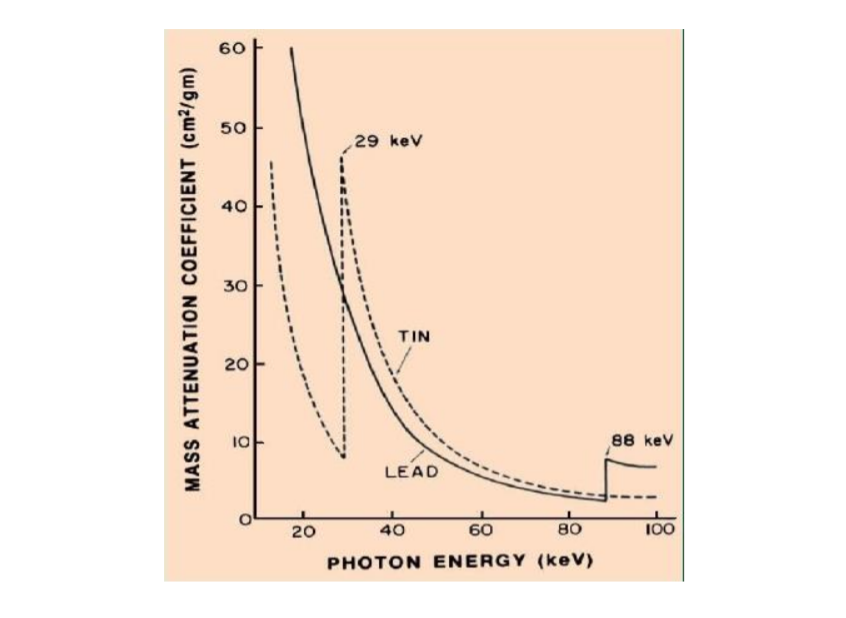
\includegraphics[width=0.80 \textwidth]{./images/NKK2.png}}
		\end{center}
		\begin{center}
			Figure: Mass attenuation coefficient for Lead and Tin
		\end{center}
		\subsection{Factors affecting attenuation}  
		The following factors affect attenuation process:\\\bigskip
		
		1. \textbf{Energy of radiation:}\\\bigskip
		As the energy of radiation increases, the number of transmitted photons increases and hence attenuation decreases.\\\bigskip
		2. \textbf{Density of the matter:}\\\bigskip
		Tissue density is one of the most important factors in Xray
		attenuation. Attenuation increases linearly with density of the matter. If the density of a material is doubled, attenuation also doubles.\\\bigskip
		3. \textbf{Effects of electrons per gram:}\\\bigskip
		If the electrons per gram of absorber increases, the number of transmitted photons decreases and hence attenuation increases.\\\bigskip
		4. \textbf{Atomic number:}\\\bigskip
		The atomic number of the absorber has the same effect on attenuation as that of density,i.e., the attenuation increases as the atomic number increases.
		
	\end{flushleft}
	\pagebreak
	\section{Demodulation}
	\begin{flushleft}
		Demodulation is the process of extracting useful original information-bearing signal that had been modulated with a carrier wave. A demodulator is a device with the help of which we recover this signal. It could be an electronic circuit in case of software-defined radios it could be a computer program also, that is used to recover the information content from the modulated carrier wave.\\\smallskip
		Since, there are many different types of modulation processes there are many types of demodulation processes as well. The signal output form a demodulator may represent the form of signal sent in the message signal, for example audio, video signals or some sort of binary data. There are mainly two different types of modulation and hence we will be discussing the demodulation in these two domains.
		\subsection{Amplitude Demodulation}
		\begin{flushleft}
			For amplitude demodulation there are a lot of methods a few of them are:
			\begin{itemize}
				\item{Envelope Detector/Demodulator}
				\item{Square Law Demodulator}
				\item{Synchronous Detector}
			\end{itemize}
			\subsubsection{Envelope Detector/Demodulator}
			\begin{flushleft}
				The circuitry for demodulation of an Amplitude Modulated wave is given as follows:
				\begin{center}
					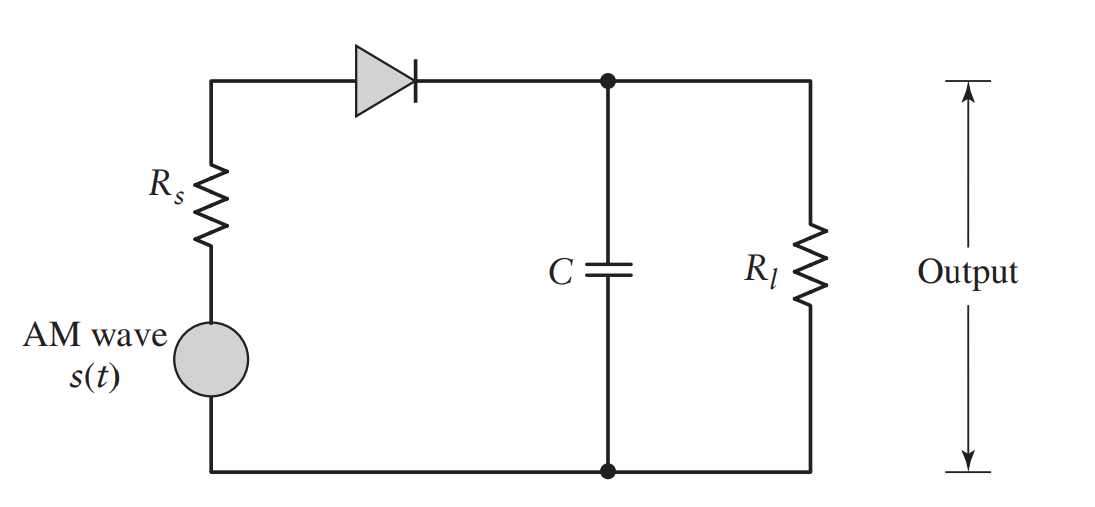
\includegraphics[width=0.60 \textwidth]{./images/Envelope Detector.png}
				\end{center}
				From the above we see how the diode in the circuit gets forward biased during the positive half of the signal and allows the capacitor to get fully charged. The discharge of capacitor during the downfall of the carrier signal help in restoration process of the original envelope of the signal. Therefore, this makes the time constant factor $\tau = R_l C$ to be just right so that the original signal is recovered. The ideal value of the factor $ \tau $ is given by the following equation,
				\begin{equation}
				\dfrac{1}{f_c} \ll R_l C \ll \dfrac{1}{f_m}
				\end{equation}
				The amplitude modulated wave is given by the following equation,
				\begin{center}
					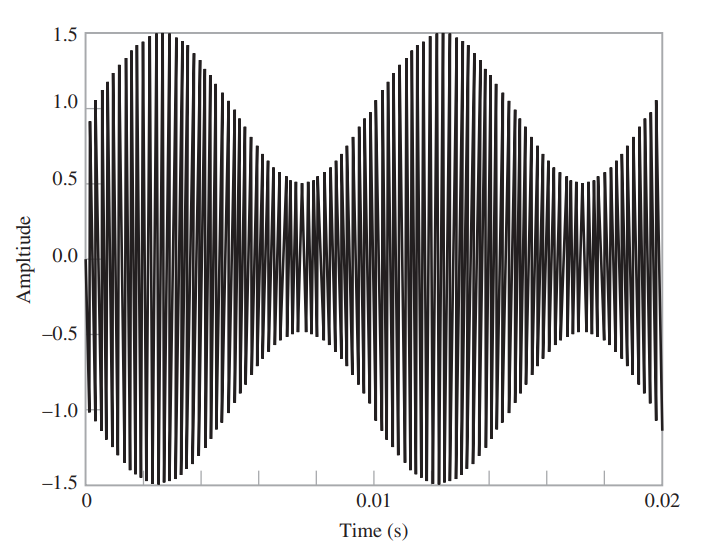
\includegraphics[width=0.60 \textwidth]{./images/ammod.png}
				\end{center}
				Passing through the circuitry shown we have the following output,
				\begin{center}
					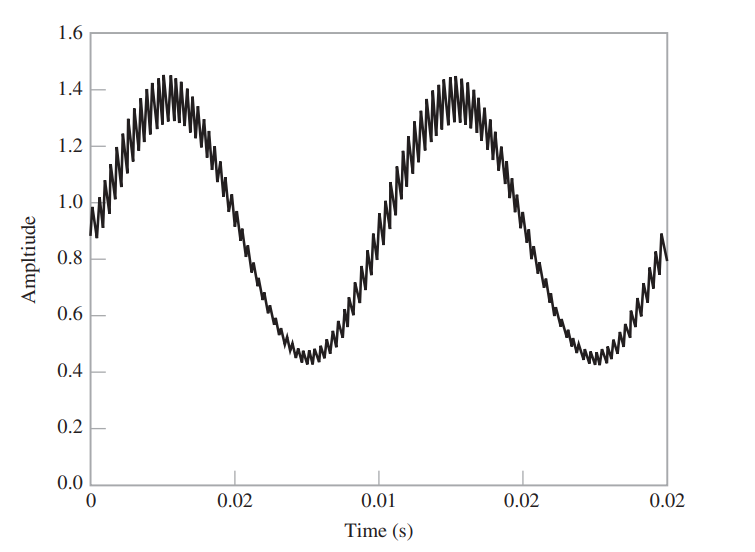
\includegraphics[width=0.60 \textwidth]{./images/amdemod.png}
				\end{center}
				If we take a look at the graph above we see that it is roughly a sinusoidal signal and will serve our purpose.\\
				Next we will be looking at the \textit{square law demodulator}.
				
			\end{flushleft}
			\subsubsection{Sqaure Law Demodulator}
			\begin{flushleft}
				\begin{center}
					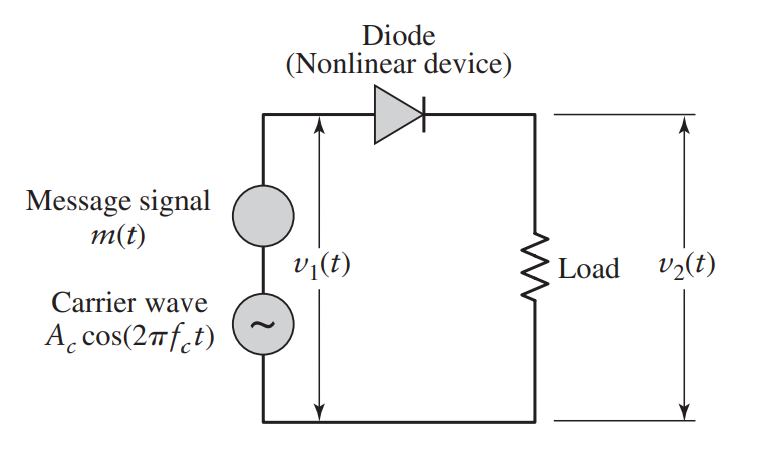
\includegraphics[width=0.60 \textwidth]{./images/Non Linear System.png}
				\end{center}
				\begin{center}
					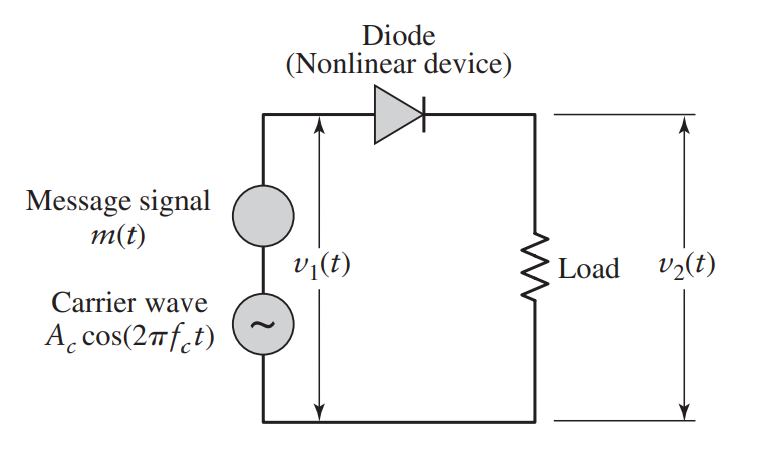
\includegraphics[width=0.60 \textwidth]{./images/Non Linear System.png}
				\end{center}
				The above figure represents a Non-Linear System that will be used to demodulate an Amplitude Modulated Signal. The block diagram of which is shown below.
				\begin{center}
					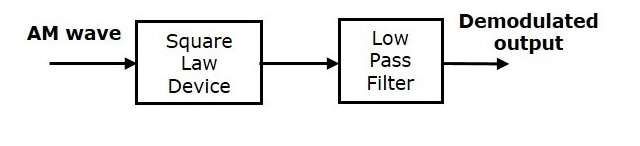
\includegraphics[width=0.60 \textwidth]{./images/Block Diagram of square law demodulator.png}
				\end{center}
				This demodulator contains a square law device as shown and low pass filter. The AM wave $V_1 (t)$ is applied as an input to this demodulator.\\
				The standard form of AM wave is,\\
				\begin{center}
					$V_1 (t) = A_c [1+k_a m(t)]cos(2 \pi f_c t)$
				\end{center} 
				We know that the mathematical relationship between the input and the output(\textit{where the output of the device is} $V_2 (t)$) of square law device is \\
				\begin{equation}
				V_2 (t) = k_1 V_1 (t) + k_2 V_1 ^ {2} (t)
				\end{equation}
				\begin{equation}
				\implies V_2 (t) = k_1 ( A_c [1+k_a m(t)]cos(2 \pi f_c t) ) + k_2 ( A_c [1+k_a m(t)]cos(2 \pi f_c t) (t) ) ^ {2} 
				\end{equation}
				Using the identity, $cos(2\theta)=2cos^{2}\theta -1$ and simplifying we have,
				\begin{center}
					$\implies V_2 (t) = k_1 A_c cos(2 \pi f_c t) ) + k_1 A_c k_a cos(2 \pi f_c t) ) + \dfrac{k_2 A_c ^2}{2}  
					$\\$+ \dfrac{k_2 A_c ^2}{2} cos(4 \pi f_c t) + \dfrac{k_2 A_c ^2 k_a^2 m^2 (t)}{2} cos(4 \pi f_c t)$\\$ + k_2 A_c^2 k_a m(t) + k_2 A_c^2 k_a m(t) cos(4 \pi f_c t)$
				\end{center}
				In the above equation, the term $k_2 A_c^2 k_a m(t)$ is the scaled version of the message signal. It can be extracted by passing the above signal through a low pass filter and the DC components can be eliminated with the help of Low Pass Filter(LPF).
				\subsection{Frequency Demodulation }
				\begin{flushleft}
					Here also in frequency modulation there are a lot of demodulation techniques to discuss a few we have,\\\smallskip
					\begin{itemize}
						\item{Frequency discrimination method.}
						\item{Phase discrimination method.}
					\end{itemize}
					\subsubsection{Frequency Discrimination Method}
					\begin{flushleft}
						We know that the standard equation of FM is given by,\\
						$s\left ( t \right ) =A_c \cos \left ( 2 \pi f_ct+2 \pi k_f \int m\left ( t \right )dt \right )$
						where,$k_f$ is the change in frequency per unit voltage of the message.\\
						$m(t)$ is the message signal\\
						others are standard parameters already defined in the frequency modulation section.\\
						Differentiating the above equation \textit{w.r.t} $t$ we have,
						\begin{equation}
						\frac{ds\left ( t \right )}{dt}= -A_c\left ( 2 \pi f_c+2 \pi k_fm\left ( t \right ) \right ) \sin\left ( 2 \pi f_ct+2 \pi k_f\int m\left ( t \right )dt \right )
						\end{equation} 
						Using the identity $-sin(\theta)=sin(\theta-\ang{180} )$
						\begin{equation}
						\implies \frac{ds(t)}{dt}=A_c\left ( 2 \pi f_c+2 \pi k_fm\left ( t \right ) \right )\sin\left ( 2 \pi f_ct+2 \pi k_f \int m\left ( t \right )dt-180^0  \right )
						\end{equation}
						\begin{equation}
						\implies \frac{ds(t)}{dt}=A_c\left ( 2 \pi f_c \right )\left [ 1+\left ( \frac{k_f}{k_c} \right )m\left ( t \right ) \right ] \sin\left ( 2 \pi f_ct+2 \pi k_f\int m\left ( t \right )dt-180^0 \right )
						\end{equation}
						The amplitude term in the above equation, resembles to that of the envelope of the AM wave, and the angle term \textit{i.e.,} the sine quantity represents the angle term of the FM wave.\\\smallskip
						Hence, our requirement is the modulating signal $m(t)$. Hence, we can recover it using envelope detector of the AM wave. The, block diagram of the Demodulator is shown as follows:
						\begin{center}
							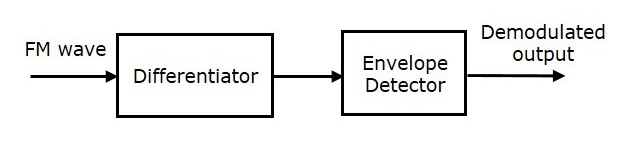
\includegraphics[width=0.60 \textwidth]{./images/Frequency Discrimination method.png}
						\end{center}
						As we can see from the block diagram we see that it consists of the differentiator and the envelope detector. Differentiator is used to convert the Frequency Modulated wave into a combination of AM and FM wave. It converts the frequency variations of FM wave into the corresponding voltage (\textit{amplitude}) variations of AM wave. We know the operation of the envelope detector as it was previously discussed in the Amplitude Demodulation section. It produces the demodulated output of the AM wave, which is our required message signal.
					\end{flushleft}
					\subsubsection{Frequency Discrimination Method}
					\begin{flushleft}
						The following diagram illustrates the FM demodulator using phase discrimination method.
						\begin{center}
							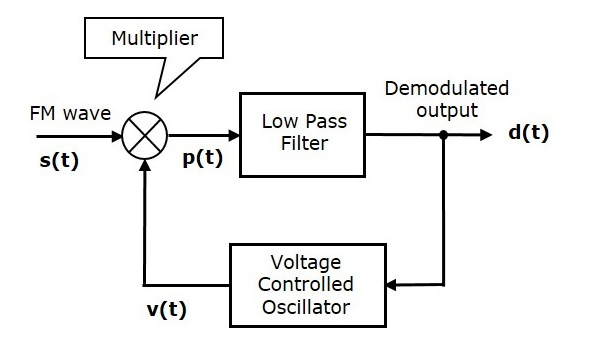
\includegraphics[width=0.60 \textwidth]{./images/Phase discrimination method.png}
						\end{center}
						From the block diagram we see that, it consists of the multiplier, the low pass filter and the Voltage Controlled Oscillator(VCO). VCO produces an output signal $v(t)$, whose frequency is proportional to the signal voltage $d(t)$. \\\smallskip
						Initially when the signal $d(t)$ is zero, adjust the VCO to produce an output signal $v(t)$, having a carrier frequency and -\ang{90} phase shift with respect to the carrier signal.\\\smallskip
						FM wave $s(t)$ and the VCO output $v(t)$ are applied as inputs of the multiplier. The multiplier produces an output, having a high frequency component and a low frequency component. Low pass filer eliminates the high frequency components and produces only the low frequency component as its output.\\\smallskip
						This low frequency component contains only the term-related phase difference. Hence we get our desired message signal.
					\end{flushleft}
				\end{flushleft}
			\end{flushleft} 
		\end{flushleft}
	\end{flushleft}
	\pagebreak
 	
\end{document}